\chapter{Traffic models}
	\section{Introduction to traffic simulators}
		One of the main branch of the traffic simulators are the so called macroscopic or hydrodynamic models. These deal with traffic as a fluid flow and they do not take individual driver actions into consideration, namely, they are based on the vehicle density.

		The other type of simulators use the microscopic or car following models. These models take individual driver behavior into consideration. So they are simulating each cars in a particular traffic situation. Two examples of these car following models are the optimal velocity model and velocity difference model.

		In this thesis the second type will be investigated since the goal is that every car should be simulated as realistic as possible which cannot be expected from the first type. Then from the experience a new model should be developed which consists the longitudinal and transversal movement models. Based on the literature review it seems that one of the most widespread microscopic model is the Intelligent Driver Model (IDM) \cite{arne1} - \cite{modified}. IDM is an excellent start for the longitudinal model.
	\section{Intelligent Driver Model} \label{sec:IDM}
		IDM is a time continuous car following model which belongs to the Optimal Velocity model family. IDM is designed to be accident-free. It can only represents longitudinal motions. The fundamental idea behind the model is that every car chooses its speed based on the car before and its individual parameters. In case when there is no car before then it can freely accelerate to its desired speed.

		IDM is defined by its acceleration function. The model is constructed by two parts. The first part represents the \textit{free acceleration} when there is no leading car or it is far away:
		\begin{equation}
			\afree=\amax\left [ 1 - \left ( \frac{\vt}{\vd} \right )^{\delta} \right ]\,,
			\label{eq:afree}
		\end{equation}
		where
		\begin{itemize}
			\item $\amax$ $\rm [m/s^2]$ is the maximum acceleration of the vehicle,
			\item $\vt$ $\rm [m/s]$ is the velocity of the vehicle at $t$,
			\item $\vd$ $\rm [m/s]$ is the desired velocity of the vehicle,
			\item $\delta$ $\rm [-]$ is the free acceleration exponent of the vehicle.
		\end{itemize}
		Equation \eqref{eq:afree} produces zero when the current speed equals to the desired speed ($\vt=\vd$) and it reaches its maximum value when the car is not moving ($\vt=0$).

		The second part corresponds to the \textit{follower behavior} or \textit{breaking strategy} of the model:
		\begin{equation}
			\afollower=-\amax\cdot \left ( \frac{\hd}{\h} \right )^2\,,
			\label{eq:afollower}
		\end{equation}
		where
		\begin{itemize}
			\item $\hd$ $\rm [m]$ is the desired safe headway of the vehicle at $t$,
			\item $\h$ $\rm [m]$ is the current headway of the vehicle at $t$.
		\end{itemize}
		The desired safe headway can be calculated from:
		\begin{equation}
			\hd=h_0 + \vt\cdot T + \frac{\vt\cdot(\vt-\vleader)}{2\sqrt{\amax\cdot\bmax}}\,,
		\end{equation}
		where $h_0$ is the bumper to bumper gap or jam distance, $T$ is the desired safety time headway, $\vleader$ is the velocity of its leader car, $\bmax$ is the maximum value of comfortable deceleration.
		The current headway at a given $t$ can be calculated from:
		\begin{equation}
		\h=\posleader-\lengthleader- x(t)
		\end{equation}
		where $x(t)$ is the position of the car, $\posleader$ and $\lengthleader$ is the position and length of the car's leader vehicle.
		Equation \eqref{eq:afollower} will decreases with increasing own speed, increasing velocity difference and decreasing distance to the front car.
		\begin{figure}
			\centering
			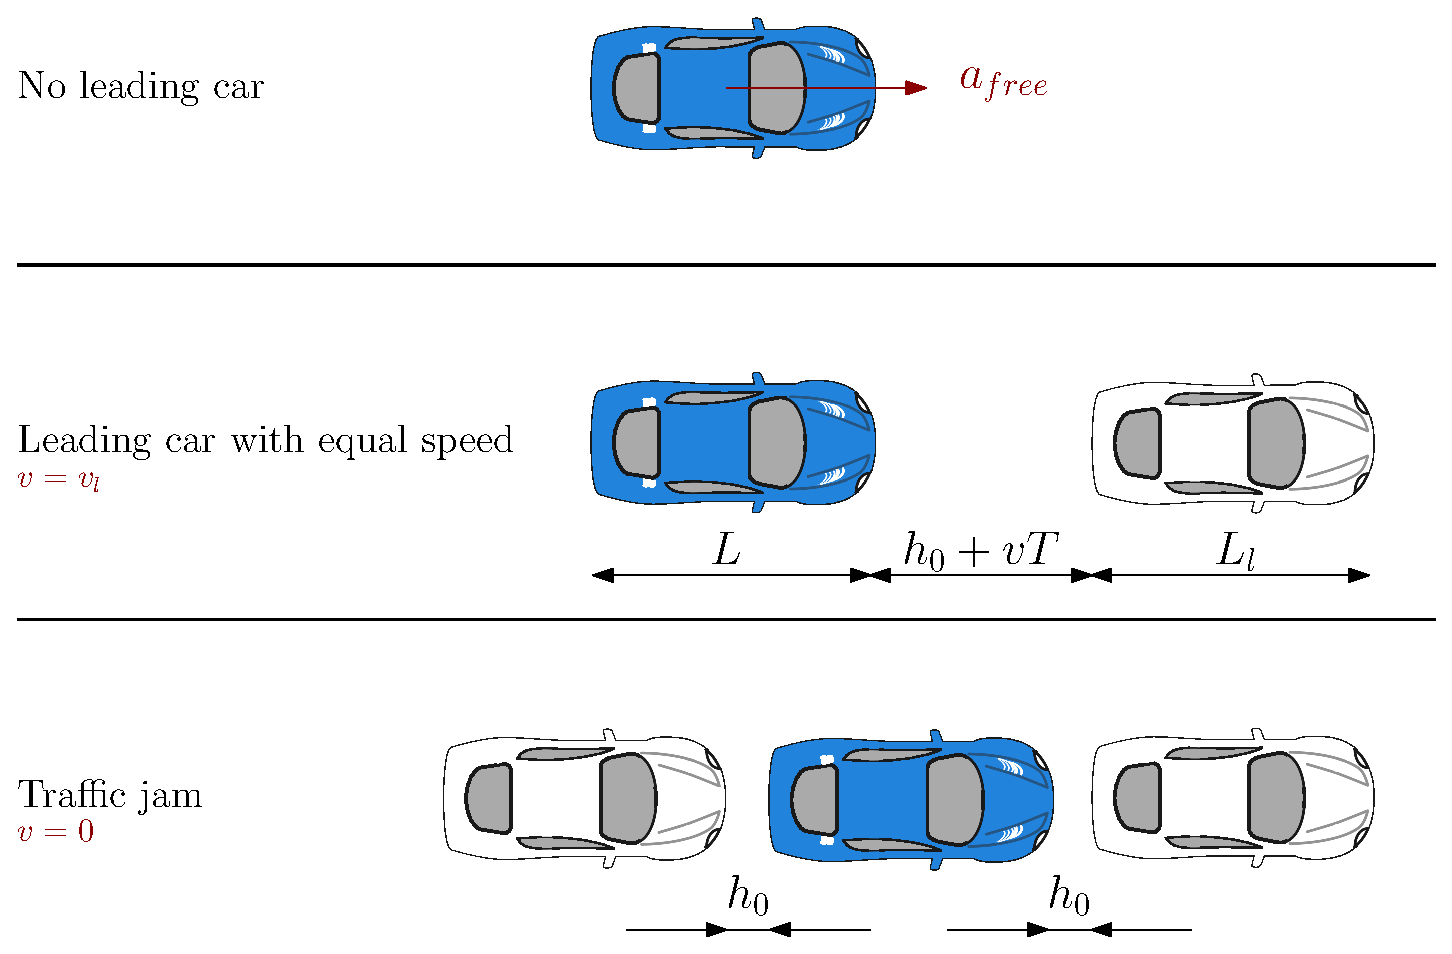
\includegraphics[width=.95\textwidth]{common/idm}
			\caption{3 cases of IDM}
			\label{fig:idm}
		\end{figure}
		The sum of Eq. \eqref{eq:afree} and \eqref{eq:afollower} is the IDM equation which reads as follows:
		\begin{equation}
			a(t)=\afree+\afollower=\amax\left [ 1 - \left ( \frac{\vt}{\vd} \right )^{\delta} - \left ( \frac{\hd}{\h} \right )^2 \right ]\,.
			\label{eq:aidm}
		\end{equation}
		Equation \eqref{eq:aidm} represents the longitudinal behavior mechanism of a human driven car. 3 cases of traffic situation were drawn on figure \ref{fig:idm} with their representative parameters.
	\section{MOBIL -- lane changing model} \label{sec:MOBIL}
		As mentioned in section \ref{sec:IDM}, there is a need for transversal motion model of the cars, namely a lane changing model. It has not been studied nearly as exhaustive as longitudinal behaviors. However it can have great impact on the overall traffic flow so it is worth investigating. The model should be able to decide based on the local traffic conditions that changing lane is beneficial and safe to a specific driver or not. If both conditions met the model will start to change lanes.

		The first condition to satisfy is that lane changing should be safe. The model should check that how will a possible lane change effect the upstream vehicles in the target lane. MOBIL \cite{arne2} states if the deceleration of the new follower car does not exceed a given safe limit then changing lanes is safe. It can be expressed with an inequality as well:
		\begin{equation}
			\hat{a}_{n}\geq -b_{\rm safe}\,,
		\end{equation}
		where $\hat{a}_{n}$ is the new follower car's acceleration if car $c$ changes lanes and $b_{\rm safe}$ is a parameter of car $n$. This criterion ensures that the model remains accident free even for edge cases.
			\begin{figure}
				\centering
				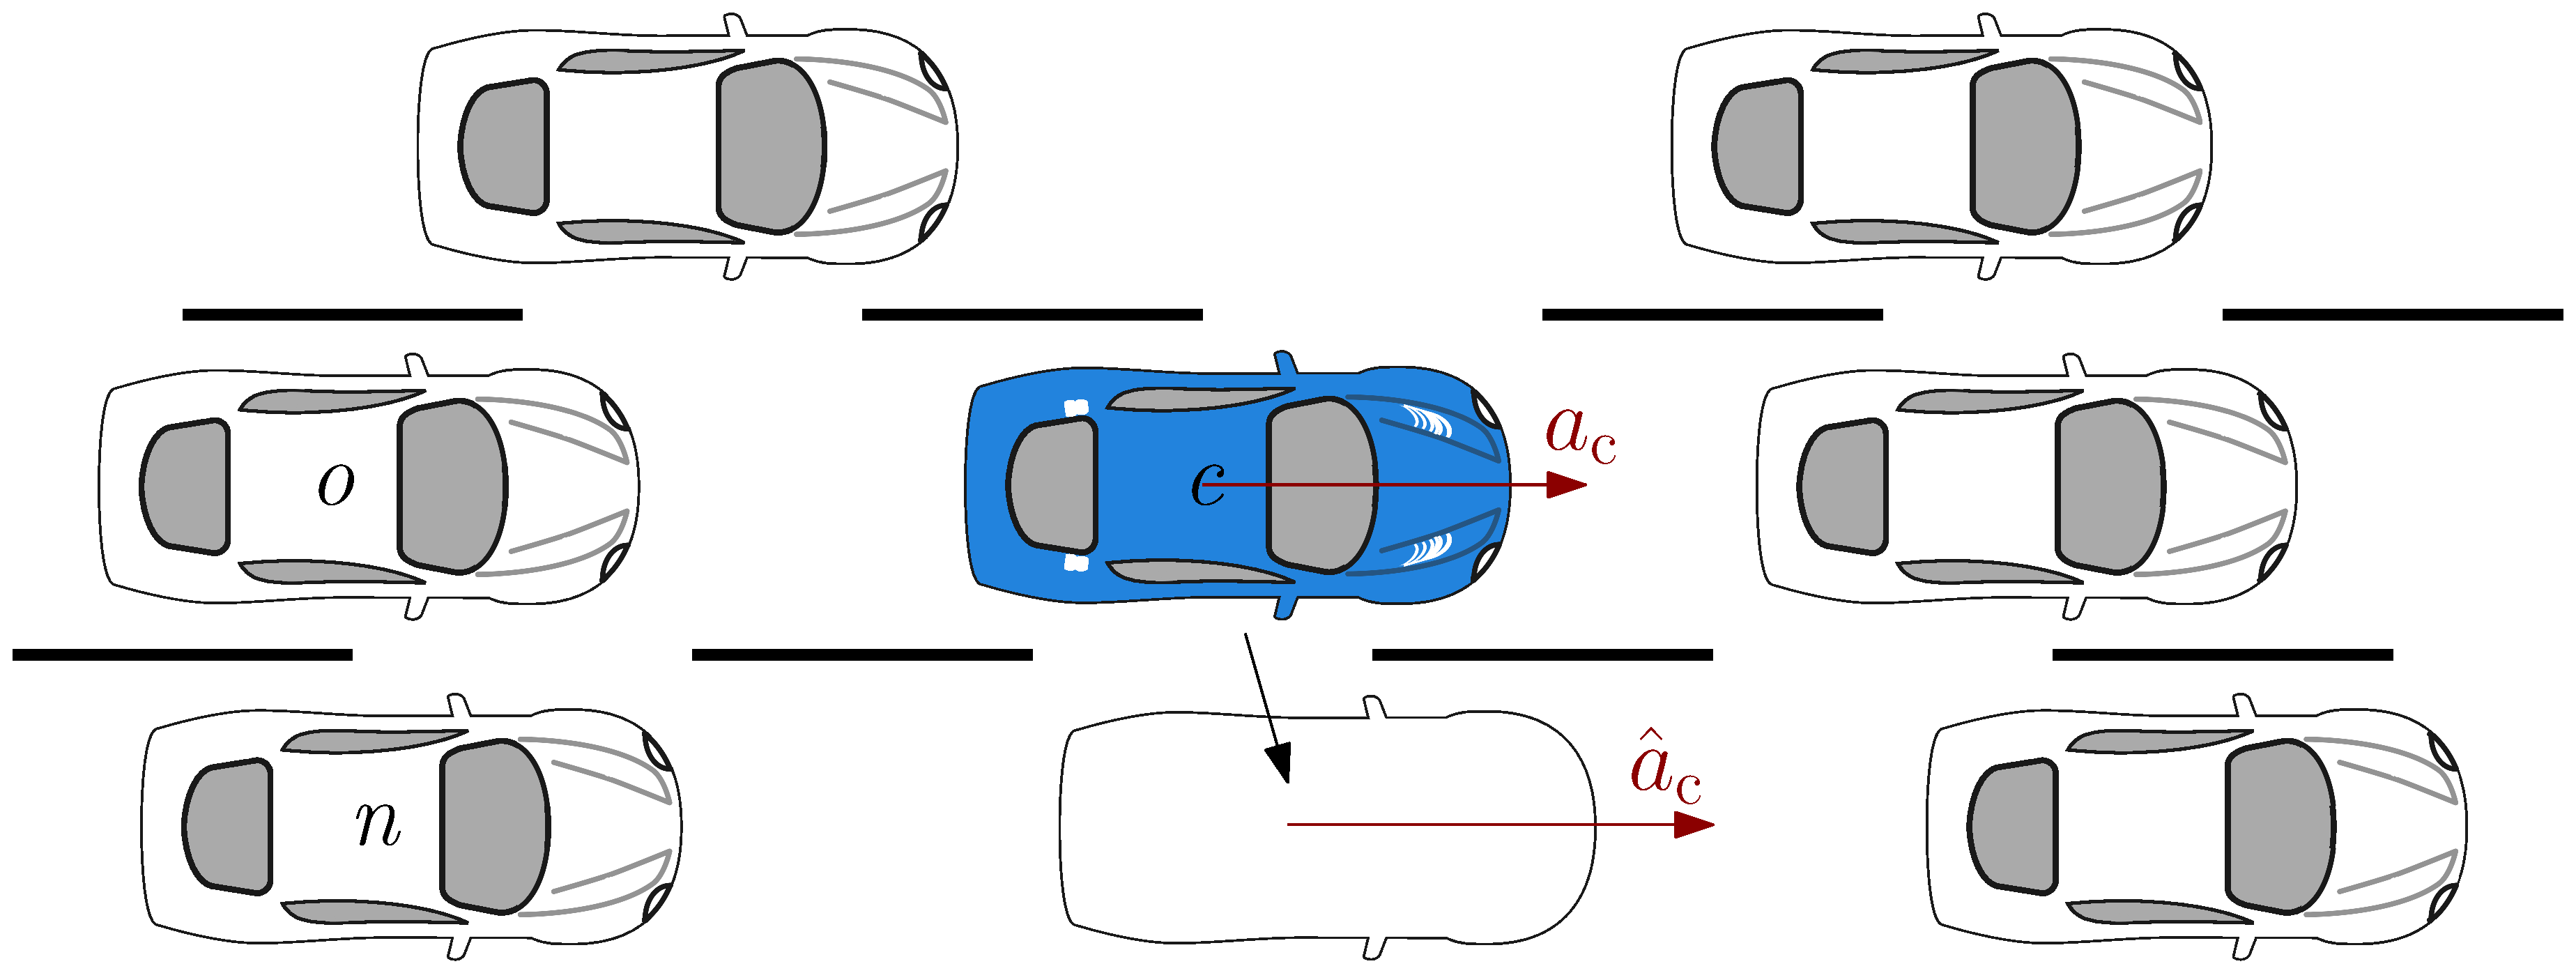
\includegraphics[width=.95\textwidth]{common/mobil}
				\caption{Based on the local traffic conditions vehicle \textit{c} is considering changing lanes to the right. Vehicle \textit{n} and \textit{o} will be the new and old followers of car \textit{c} respectively.}
				\label{fig:mobil}
			\end{figure}
			The other condition is the incentive criterion which states that the lane change should improve the local traffic situation around the vehicle. The base model is the following:
			\begin{equation}
				\hat{a}_{\rm c} + \hat{a}_{\rm o} + \hat{a}_{\rm n} > a_{\rm c} + a_{\rm o} + a_{\rm n}\,,
				\label{eq:mobil_first}
			\end{equation}
			where accelerations after a possible lane change are denoted with caps.
			Based on Eq. \eqref{eq:mobil_first} a lane change should occur only if the sum of the accelerations after the lane change is greater than before. This inequality reflects the name of the model which is \textbf{m}inimizing \textbf{o}verall \textbf{b}raking \textbf{i}nduced by \textbf{l}ane change.

			However Eq. \eqref{eq:mobil_first} is not as realistic as it should be. The first problem is that vehicles would change lanes even for a negligible acceleration advantage which is not the case in a realistic traffic situation. This issue can be solved with a threshold value $\Delta a_{\rm th}$. After this modification Eq. \eqref{eq:mobil_first} would look like below:
			\begin{equation}
				\hat{a}_{\rm c} - a_{\rm c} + \hat{a}_{\rm o} - a_{\rm o} + \hat{a}_{\rm n} - a_{\rm n} > \Delta a_{\rm th}\,,
				\label{eq:mobil_with_tr}
			\end{equation}
			It can be stated that with this modification individual drivers only change lanes if the acceleration sum is significantly greater than before the lane change. The other problem with the previously discussed model is that they can't distinguish between driving style. Driver styles can vary from complete selfish to the altruistic driver. Selfish drivers would only care about their own acceleration ($\hat{a}_{\rm c} - a_{\rm c} > \Delta a_{\rm th}$) while altruistic ones would change lanes even if that would result in a disadvantageous position for them but with that change the local traffic situation would improve sufficiently ($\hat{a}_{\rm o} - a_{\rm o} + \hat{a}_{\rm n} - a_{\rm n} > \Delta a_{\rm th}$). A $p$ politeness factor should be introduced to fix that. Including $p$ in Eq. \eqref{eq:mobil_with_tr} results in the final form of the model:
			\begin{equation}
				\hat{a}_{\rm c} - a_{\rm c} + p(\hat{a}_{\rm o} - a_{\rm o} + \hat{a}_{\rm n} - a_{\rm n}) > \Delta a_{\rm th}\,.
				\label{eq:mobil}
			\end{equation}
			A completely selfish driver would get $p=0$ factor, while an altruistic one $p>1$. In the special case where $p=1$ Eq. \eqref{eq:mobil} simplifies back to Eq. \eqref{eq:mobil_with_tr}, which means a lane change is performed only if the sum of all involved vehicles' acceleration will improved at least by the threshold value.
		\section{Numerical solver}
			In Section \ref{sec:IDM} and \ref{sec:MOBIL} a vehicle behavior in traffic has been shown and modeled. The mathematical model of a driver is a second order differential equation. There is no analytical solution, so a numerical one should be carried out. To be able to use one of the common numerical solvers (like Explict Euler or 4th order Runge Kutta) the second order differential equation should be transformed into a first order differential equation system. So the second order differential equation to solve based on Eq. \eqref{eq:aidm} and the facts that $v=\dot{x},\,a=\ddot{x}$, will be the following:
			\begin{equation}
				\ddot{x}=\amax\left [ 1 - \left ( \frac{\dot{x}}{\vd} \right )^\delta - \left ( \frac{h_0 + \dot{x}\cdot T + \frac{\dot{x}(\dot{x}-v_{\rm lead})}{{\rm c}}}{x_{\rm lead}-L_{\rm lead} - x} \right )^2 \right ]\,.
				\label{eq:idm_num1}
			\end{equation}
			Let's say
			\begin{equation}
				\textbf{y}=
				\begin{pmatrix}
					y_1\\
					y_2
				\end{pmatrix}
				=
				\begin{pmatrix}
					x\\
					\dot{x}
				\end{pmatrix}\,,
				\label{eq:idm_num2}
			\end{equation}
			then the derivative of $\textbf{y}$ would be
			\begin{equation}
				\dot{\textbf{y}}=
				\begin{pmatrix}
					\dot{y_1}\\
					\dot{y_2}
				\end{pmatrix}
				=
				\begin{pmatrix}
					\dot{x}\\
					\ddot{x}
				\end{pmatrix}\,,
				\label{eq:idm_num3}
			\end{equation}
			From Eq. \eqref{eq:idm_num1}, \eqref{eq:idm_num2} and \eqref{eq:idm_num3} it can be concluded that the differential equation system will be the following:
			\begin{equation}
				\dot{\textbf{y}}
				=
				\begin{pmatrix}
					f_1(y_2)\\
					f_2(y_1,y_2,x_{\rm lead},v_{\rm lead})\\
				\end{pmatrix}
				=
				\begin{pmatrix}
					y_2\\
					\amax\left [ 1 - \left ( \frac{y_2}{\vd} \right )^{\delta} - \left ( \frac{h_0 + y_2\cdot T + \frac{y_2(y_2-v_{\rm lead})}{{\rm c}}}{x_{\rm lead} - L_{\rm lead} - y_1} \right )^2 \right ]
				\end{pmatrix}
				\label{eq:numerical_idm}
			\end{equation}